%% CAPITULO 3
\hypertarget{estilo:capitulo}{}
\chapter{IMPACTO DA ASSIMILAÇÃO DE PRECIPITAÇÃO NO SISTEMA Eta+RPSAS}

\section{Avaliação das médias dos experimentos durante Janeiro de 2003}
\label{ss:avalmedia}

Dois experimentos com e sem a inclusão de precipitação do TRMM (denominados CAP e SAP, respectivamente) no sistema Eta+RPSAS foram realizados com o objetivo de se verificar o impacto produzido pela assimilação de precipitação nas análises geradas pelo sistema RPSAS e nas previsões geradas pelo modelo Eta.

Para se verificar o comportamento desses experimentos ao longo do período de integração do modelo (de 02 a 30 de Janeiro de 2003), foi feita uma avaliação espacial média da integração do modelo durante o período de estudos em comparação com as reanálise 2 do NCEP/DOE e a reanálise do CPTEC. Para esta avaliação foram consideradas as análises do sistema RPSAS em um total de 113 análises (entre 00Z, 06Z, 12Z e 18Z), considerando-se também  o período de spin up, a partir das quais foi feita a média espacial para o domínio de integração do modelo. Todos os campos considerados nesta avaliação espacial (incluindo-se a reanálise do CPTEC) foram interpolados para a grade da reanálise do NCEP. Na seção X são apresentas as avaliações das Análises do sistema RPSAS contra as Reanálises do CPTEC e do NCEP. Foram avaliadas as variáveis de Temperatura Absoluta, Ventos (u+v), Altura Geopotencial e Circulação do Vento (Linha de Corrente) nos níveis de 850, 500 e 250 hPa. Também, foram verificadas separadamente as componente zonal do vento (u) em 250 hPa e meridional (v) em 850 hPa, além da Temperatura a dois metros. Na seção XX são apresentas as avaliações das previsões do modelo Eta contra as observações do SALLJEX e do TRMM. Esta avaliação é feita para as mesmas variáveis.

\subsubsection{Avaliação das Análises (Análises RPSAS X Reanálises)}

A Figura 1.1 mostra os campos médios de Linha de Corrente para o nível de 850 hPa. Em a) tem-se o experimento SAP, em b) o experimento CAP, em c) a Reanálise do CPTEC e em d) a Reanálise 2 do NCEP/DOE. Comparando-se os dois experimentos (SAP e CAP), nota-se que em ambas as simulações o padrão de escoamento é semelhante a partir do qual pode-se observar um gradiente do escoamento de leste sobre o Atlântico Subtropical e outro de oeste sobre o norte da AS. Em relação à reanálises, a do CPTEC também apresenta estes dois gradientes com um padrão de circulação mais organizado apresentando também um giro bem definido sobre o Atlântico Subtropical dando suporte a esse escoamento de leste. Na reanálise do NCEP também  observa-se esta confluência do escoamento de leste sobre o Atlântico Subtropical, e também o de oeste sobre o Norte da AS, porém um pouco menos intenso. Ambos os experimentos tenderam a simular uma circulação ao centro do continente, sendo esta mais bem caracterizada no experimento CAP. Este tipo de circulação não foi simulado pelas reanálises. PORQUE ACHA QUE NÃO FOI ENCONTRADA NAS REANALISES, CICLONICA OU ANTICICLONICA, VERIFICAR A PRECIPITACAO. Em todos os casos  observar-se o fluxo zonal ao sul da AS em 850 hPa.

\begin{figure}[!hbp]
\centering
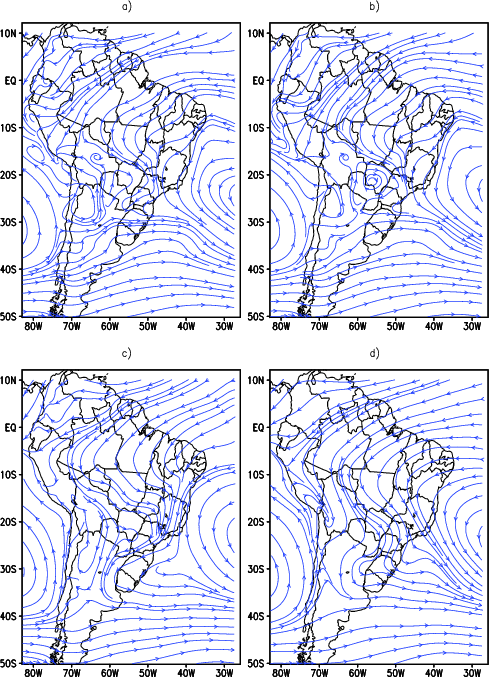
\includegraphics[height=15cm]{./figs/media_corrente_anl_850hPa.png}
\caption{Linha de Corrente para o nível de 850 hPa. a) experimento SAP, b) experimento CAP, c) Reanálise CPTEC, d) Reanálise 2 NCEP/DOE.}
\label{fig31}
\end{figure}

Em níveis médios (500 hPa), os experimentos SAP e CAP também apresentam um padrão de circulação semelhante entre si divergindo pouco daquele apresentado pelas reanálises. Neste nível, a reanálise do NCEP apresenta um gradiente caracterizado por um escoamento de leste no nordeste da AS. Este padrão de escoamento foi simulado pelos experimentos e pela reanálise mas, no entanto, o gradiente associado a ele não foi bem caracterizado pelo experimento CAP e foi caracterizado de forma discreta pelo experimento SAP. Em comparação ao nível de 850 hPa, os experimentos parecem ser mais concordantes com as reanálises apresentando padrões de circulação mais semelhantes a essas. Isto pode ser devido ao fato de que entre 500 e 600 hPa a atmosfera é caracterizada por ser não divergente em que assume-se que a vorticidade relativa é nula ou ainda, em que os movimentos são essencialmente verticais.

\begin{figure}[!hbp]
\centering
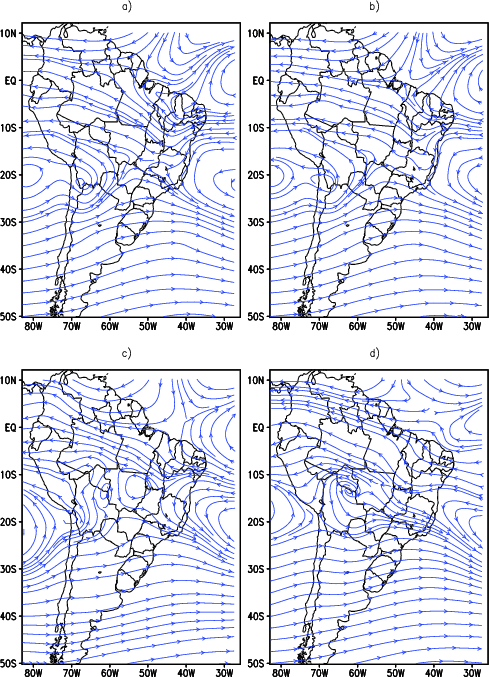
\includegraphics[height=15cm]{./figs/media_corrente_anl_500hPa.png}
\caption{Idem Figura 1.1, para o nível de 500 hPa.}
\label{fig32}
\end{figure}

No nível de 250 hPa observa-se que as médias das reanálises apresentam um vórtice de circulação anticiclônica (bem definido na reanálise do NCEP). Além disso, na reanálise do NCEP também nota-se um cavado ao norte do continente. Este cavado não fica bem caracterizado nos experimentos SAP e CAP, embora a circulação do vento seja semelhante naquele setor. No entanto, o escoamento zonal de oeste ao sul e a nordeste do continente está presente nos dois experimentos e nas duas reanálises.

\begin{figure}[!hbp]
\centering
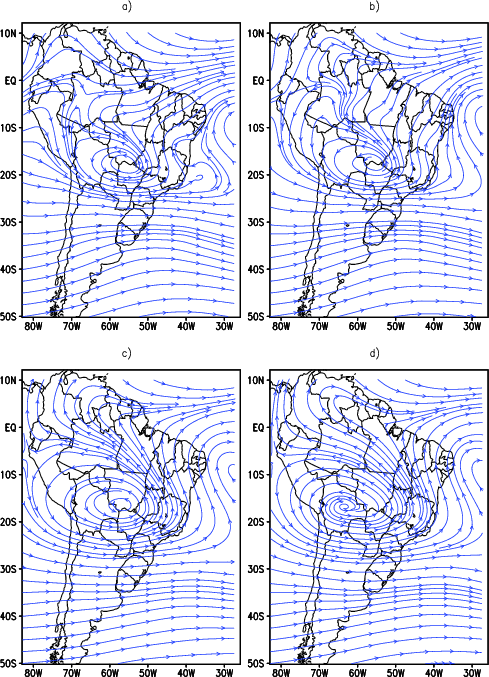
\includegraphics[height=15cm]{./figs/media_corrente_anl_250hPa.png}
\caption{Idem Figura 1.1, para o nível de 250 hPa.}
\label{fig33}
\end{figure}

As figuras a seguir mostram os campos médios da magnitude e direção do vento (u+v) durante o período de avaliação. Em 850 hPa, é possível identificar um caso de JBN que é caracterizado por ventos de norte/nordeste intensos em baixos níveis canalizado pela topografia dos Andes (bloqueio topográfico). Este tipo de jato fica bem caracterizado na média da reanálise do NCEP, devido à aceleração da componente meridional do vento, havendo um pequeno sinal de sua atuação na reanálise do CPTEC. No entanto, não há sinal aparente de sua atuação nas médias das simulações SAP e CAP. Entre outros aspectos que podem ser notados, pode-se citar que os experimentos e a reanálise do NCEP concordam sobre a intensidade do vento sobre a região norte do continente. Neste caso, a reanálise do CPTEC tende a superestimar a intensidade do vento em superfície em relação aos experimentos e reanálise do NCEP. 

Estes resultados podem estar associados às configurações adotadas para o modelo Eta nos experimentos SAP e CAP, como por exemplo a aproximação hidrostática. Outro fator que pode ter colaborado para esta disparidade entre as análises globais e regionais, é a essencia mais estatística do que dinâmica do sistema de análises RPSAS. Além disso a inclusão de precipitação pode ter causado um desbalanço entre os campos de massa e vento e o filtro digital pode não ter sido eficiente na inicialização dos dados antes da previsão e/ou após a análise. 

\begin{figure}[!hbp]
\centering
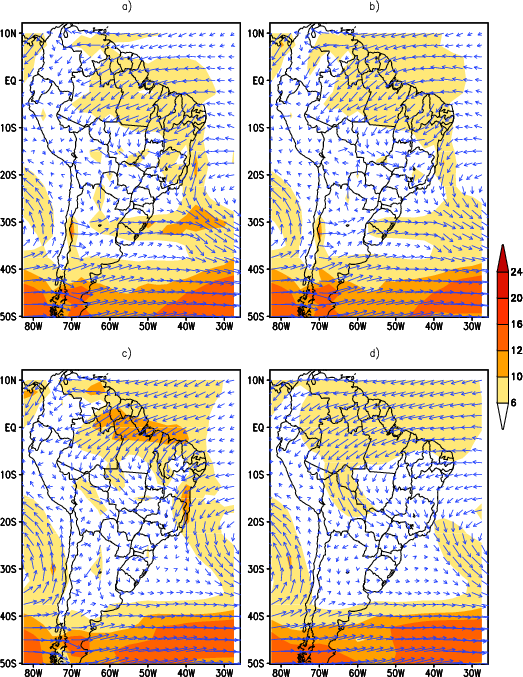
\includegraphics[height=15cm]{./figs/media_ventos_anl_850hPa.png}
\caption{Magnitude e direção do vento (u+v) para o nível de 850 hPa. a) experimento SAP, b) experimento CAP, c) Reanálise CPTEC, d) Reanálise 2 NCEP/DOE.}
\label{fig34}
\end{figure}

Em níveis médios (500 hPa), assim como em altos níveis (250 hPa), o escoamento ao sul do continente é predominantemente zonal e de oeste, característico da atuação dos jatos de Altos Níveis (Jatos Polar e Subtropical), em que a magnitude do vento permanece acima de 20 ms-1. Neste nível, não se percebe grandes diferenças entre os experimentos e as reanálises. Entre as latitudes de 20ºS e 30ºS, os experimentos SAP e CAP tendem a posicionar os Jatos de Altos Níveis em latitudes mais baixas, em relação às reanálises, que concordam sobre a posição desses jatos. VERIFICAR AS FIGURAS a E b, MUITO ESTRANHAS.

\begin{figure}[!hbp]
\centering
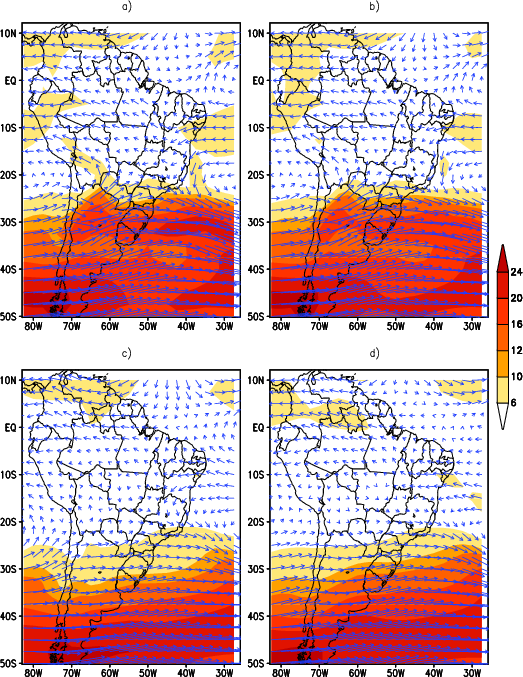
\includegraphics[height=15cm]{./figs/media_ventos_anl_500hPa.png}
\caption{Idem Figura 1.4, para o nível de 500 hPa.}
\label{fig35}
\end{figure}

Em 250 hPa, a presença dos Jatos de Altos Nível ao sul do continente é marcante e sua atuação é importante devido à influência que exercem na propagação de frentes atmosféricas e na formação de alguns sistemas convectivos. Neste nível, os experimentos SAP e CAP apresentam características semelhantes de escoamento, tando em relação à circulação quanto em relação à intensidade. O mesmo ocorre em relação às duas reanálises, sendo que a do NCEP fecha um vórtice (que pode ser visto no campo de linha de corrente da Figura X). Este vórtice não é bem caracterizado pelos dois experimentos. E MAIS INTENSA A CIRCULACAO NOS EXPERIMENTOS SAP E CAP, PORQUE. No entanto, a posição e a intensidade dos Jatos é bem definida e coerente entre os quatros campos apresentados na Figura X, com a componente zonal do vento apresentando valores máximos (acima de 24 ms-1).

\begin{figure}[!hbp]
\centering
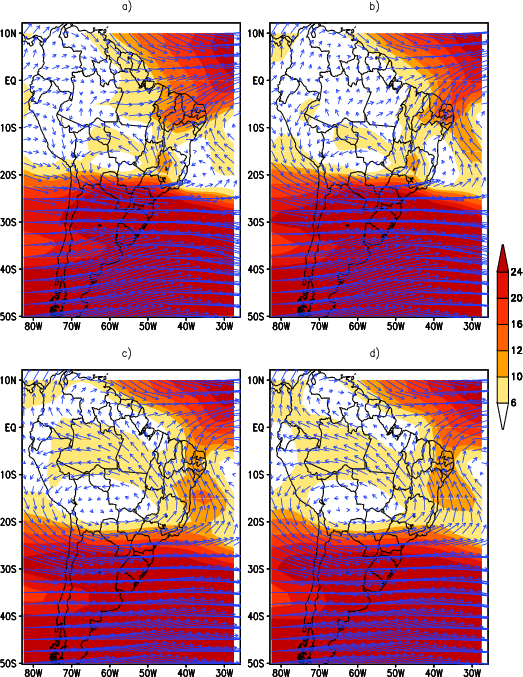
\includegraphics[height=15cm]{./figs/media_ventos_anl_250hPa.png}
\caption{Idem Figura 1.4, para o nível de 250 hPa.}
\label{fig36}
\end{figure}

Analisando-se separadamente a componente zonal do vento em 250 hPa, percebe-se que o experimento SAP tende a aumentar a magnitude da componente zonal sobre o região Nordeste do Brasil. O experimento CAP apresenta valores mais amenos desta componente do vento sobre esta região e é mais coerente com os valores apresentados pelas reanálises.

\begin{figure}[!hbp]
\centering
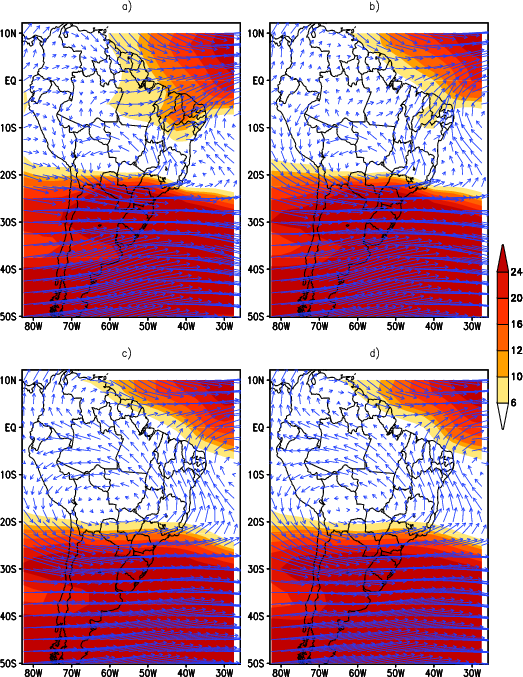
\includegraphics[height=15cm]{./figs/media_vento-zonal_anl_250hPa.png}
\caption{Componente Zonal do vento para o nível de 250 hPa. a) experimento SAP, b) experimento CAP, c) Reanálise CPTEC, d) Reanálise 2 NCEP/DOE.}
\label{fig37}
\end{figure}

A avaliação da componente meridional do vento em 850 hPa revela que os experimentos não foram muito hábeis em detectar o JBN, que é um importante componente do sistema de monção do continente e que transporta umidade da bacia amazâonia em direção à bacia do paraná-prata onde são predominantes do SCMs. A reanálise do NCEP consegue caracterizar bem a presença do jato, com a direção do vento sendo de norte e magnitude acima de 6 ms-1. A reanálise do CPTEC apresenta também um corredor de vento com as mesmas características de direção e magnitude do vento, porém menos organizado, não sendo possível dizer que há convergência dos ventos de norte tal como é bem caracterizado pela reanálise do NCEP. Os experimentos SAP e CAP, apresentam ventos fortes de sul com magnitude acima de 6 ms-1, sendo portanto, na direção contrária ao que é apresentado pelas reanálises. VERIFICAR O POR QUE DISSO, OS RESULTADOS NÃO PODEM SER MUITO DIFERENTE DA REANALISE REGIONAL, VERIFIQUE OS SCRIPTS. 

\begin{figure}[!hbp]
\centering
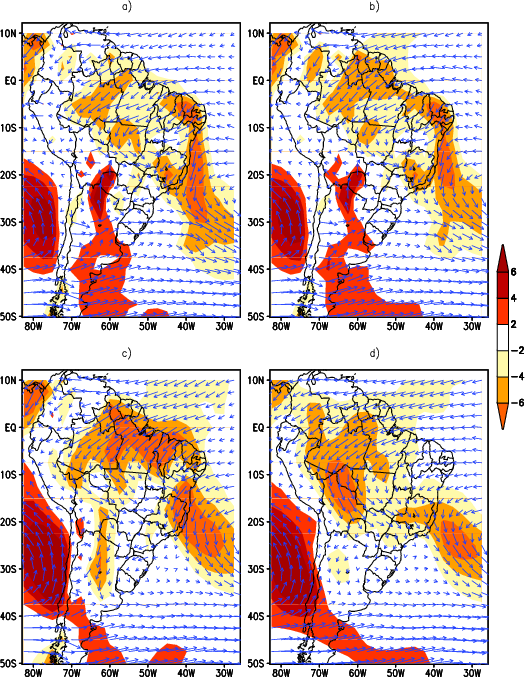
\includegraphics[height=15cm]{./figs/media_vento-meridional_anl_850hPa.png}
\caption{Componente Meridional do vento para o nível de 850 hPa. a) experimento SAP, b) experimento CAP, c) Reanálise CPTEC, d) Reanálise 2 NCEP/DOE.}
\label{fig38}
\end{figure}

A comparação entre os experimentos e as reanálises do NCEP e do CPTEC para a temperatura absoluta, mostra que para os três níveis avaliados (850, 500 e 250 hPa) as temperaturas em boa parte do continente (aproximadamente entre a faixa de latitudes de -20ºS e 10ºN, tenderam a ser mais quentes (~2ºC a mais do que as reanálises). Estas diferenças também podem ser notadas nas médias dos campos de Altura Geopotencial devido à relação existente (hipsométrica) entre temperatura e a espessura da camada acima.

\begin{figure}[!hbp]
\centering
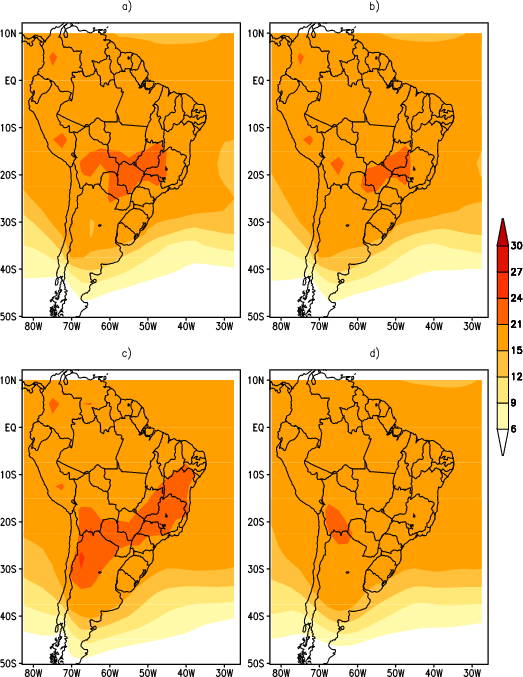
\includegraphics[height=15cm]{./figs/media_temp_anl_850hPa.png}
\caption{Temperatura Absoluta para o nível de 850 hPa. a) experimento SAP, b) experimento CAP, c) Reanálise CPTEC, d) Reanálise 2 NCEP/DOE.}
\label{fig39}
\end{figure}

\begin{figure}[!hbp]
\centering
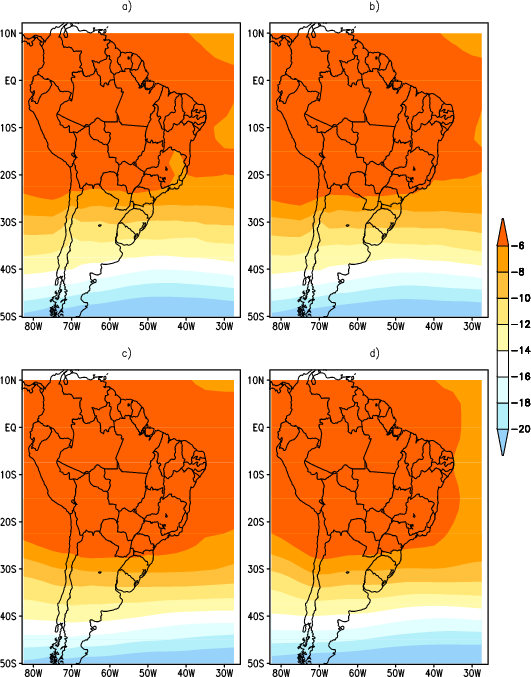
\includegraphics[height=15cm]{./figs/media_temp_anl_500hPa.png}
\caption{Idem Figura 1.9, para o nível de 500 hPa}
\label{fig40}
\end{figure}

\begin{figure}[!hbp]
\centering
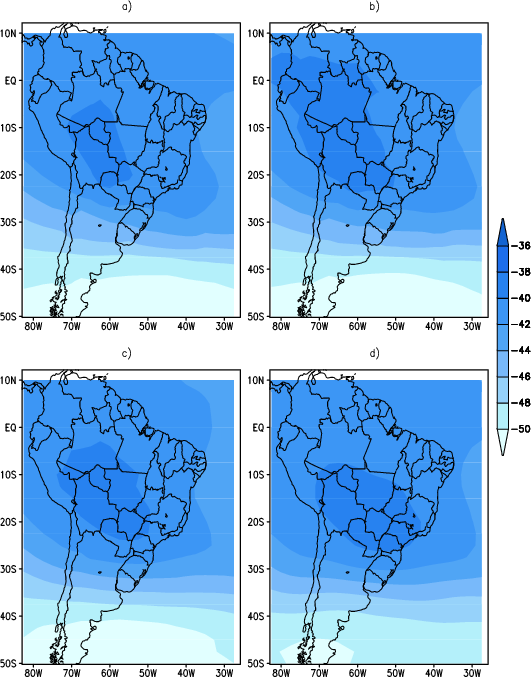
\includegraphics[height=15cm]{./figs/media_temp_anl_250hPa.png}
\caption{Idem Figura 1.9, para o nível de 250 hPa}
\label{fig41}
\end{figure}

Para a temperatura à dois metros, observa-se que o experimento SAP tende a aquecer mais a superfície no setor norte do continente do que o experimento CAP. Em relação às reanálises, observa-se que a do NCEP apresenta temperatura entre 24ºC e 27ºC, sendo que a reanálise do CPTEC tende a diminuir um pouco mais a temperatura nesse setor.  SE CONSEGUE OS DADOS DE TMP 2M DO CRU PODE COMPARAR MELHOR.

\begin{figure}[!hbp]
\centering
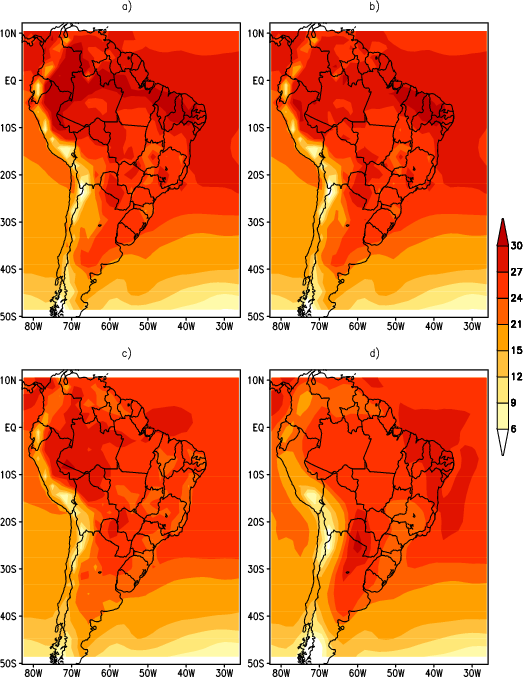
\includegraphics[height=15cm]{./figs/media_tp2m_anl.png}
\caption{Temperatura a dois metros. a) experimento SAP, b) experimento CAP, c) Reanálise CPTEC, d) Reanálise 2 NCEP/DOE.}
\label{fig42}
\end{figure}

As figuras a seguir mostram as séries do Viés e do Erro Quadrático Médio das análises em relação à reanálise do NCEP, para os níveis de 850, 500 e 250 hPa das variáveis Altura Geopotencial [mgp], Temperatura do Ar [ºC], Ventos Zonal e Meridional [ms-1] e Umidade Relativa [\%], durante 02 e 30 de Janeiro de 2003.

A avaliação das séries temporais das análises do RPSAS em relação às análises do NCEP, mostram que, em geral, os maiores valores de erro (Viés) encontram-se no nível de 250 hPa, para o experimento SAP. O experimento CAP apresenta valores de Viés menores (se comparado com o experimento SAP), sugerindo que a assimilação de precipitação tende a retirar mais o Viés em superfície (850 hPa) e em médios níveis (500 hPa) do que em altos níveis. Esta avaliação é válida para as variáveis dinâmicas do modelo, tais como ventos (zonal e meridional), temperatura e umidade. A altura geopotencial, ao contrário do que se segue para as variáveis dinâmicas, apresenta maiores diferenças de Viés e EQM para o nível de 250 hPa. Isto pode ser explicado pelo fato de que os valores de Viés e EQM da variável Temperatura do Ar apresentarem maiores diferenças entre os experimentos em baixos e médios níveis, 850 e 250 hPa. A avaliação da distribuição espacial do Viés e do EQM reforçam este ponto de vista. Para a Altura Geopotencial (Figura X), observa-se que os maiores valores de Viés e EQM estão no nível de 250 hPa e sobre a região Sul do Brasil e Argentina. Comparativamente, os experimentos SAP e CAP tenderam a subestimar a altura geométrica do Geopotencial (~30 mgp), sendo que o experimento CAP apresentou um distribuição menor do erro do que o experimento SAP. Além disso, neste mesmo nível, o experimento CAP em algumas partes da região de avaliação, removeu o Viés negativo e em outras acabou por superestimar o valor do Viés. Consequentemente, a distribuição espacial do EQM para esta variável também é maior em altos níveis. Em 850 e 500 hPa, o valor do EQM para altura Geopotencial foi menor do que em 250 hPa, nível em que a distribuição espacial do EQM foi maior e acima de 20 mgp.

A temperatura, ao contrário do que ocorreu com a Altura Geopotencial, apresentou maiores valores de Viés e EQM em superfície do que em médios e altos níveis (Figura X). Em 850 hPa, a maior parte do Viés concentrou-se na região centro-oeste do Brasil apresentando valores positivos de Viés e em poucos pontos isolados valores negativos, como sobre o a região central da Argentina. Em 500 hPa, os valores de Viés foram menores havendo um deslocamento do Viés positivo da temperatura para a região oeste do continente, porém com valores menores. Sobre a região centro-oeste do continente, os valores negativos de Viés também foram minimizados. Já em 250 hPa, os erros foram bem menore se comparados aos valores de erro em superfície (850 hPa). Neste nível, porém, observa-se que uma pequena tendência de Viés positivo sobre o oceano Atlântico Subtropical. Sobre o Norte da Argentina, e comparativamente ao experimento SAP, o experimento CAP apresentou Viés muito próximo de zero. A distribuição espacial do EQM para a Temperatura Absoluta mostra claramente que os erros mais significativos entre os experimentos foram em baixos níveis.

As componentes Zonal e Meridional do vento (Figura  X e FiguraX) avaliadas, mostram que maiores valores de Viés forma encontradas em 850 hPa e 500 hPa, respectivamente. A distribuição espacial do Viés do vento meridional nestes dois níveis é semelhante entre ambos os experimentos, sendo que o experimento CAP tende a atenuar os valores máximos e mínimos do Viés. Em boa parte do continente, ambos os experimentos tendem a subestimar o valor da componente meridional do vento. Em regiões isoladas (regiões central do continente e norte da Argentina), os experimentos superestimaram os valores do Viés. Em 250 hPa, os valores de Viés apresentados pelos experimentos tendem a ser atenuados, embora o EQM apresentado por eles seja um pouco maior do que aqueles observados em 500 e 850 hPa. Já os valores de Viés e EQM calculados para os experimentos CAP e SAP para a componente zonal do vento, mostram que há uma tendência maior dos experimentos em superestimar os valores desta componente em altos níveis. Em 500 e 850 hPa, os valores de Viés tendem a ser subestimados (~5 ms-1), sendo que sobre o norte da Argentina e sul do Brasil, estes valores são levemente superestimados.

A avaliação do Viés e EQM da umidade relativa para os níveis de 850, 500 e 250 hPa, mostra que em níveis médios (500 hPa)), os experimentos SAP e CAP foram menos tendenciosos em superestimar ou subestimar os valores relativos de umidade. Neste nível, foram encontrados menores valores de EQM. Em relação os níveis de 850 hPa e 500 hPa, houve maior tendencia dos experimentos em subestimar a umidade do ar, sendo que novamente o experimento CAP atenuou os valores do Viés e do EQM.


\begin{figure}[!hbp]
\centering
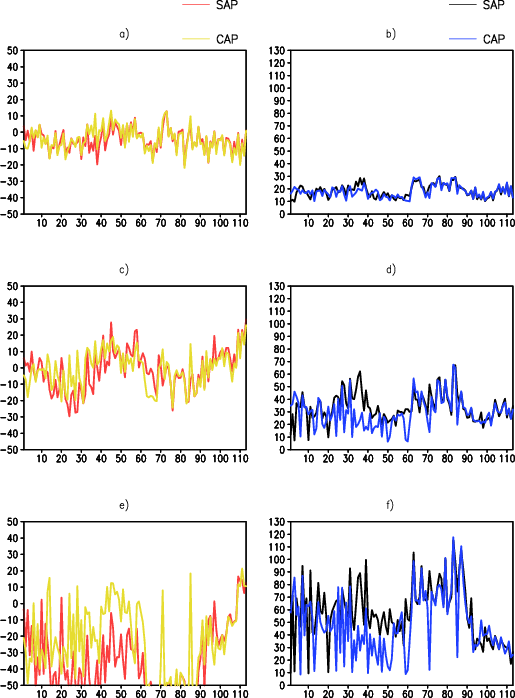
\includegraphics[height=15cm]{./figs/vies_eqm-zgeo.png}
\caption{Viés (coluna da esquerda) e Erro Quadrático Médio (coluna da direita) da Altura Geopotencial [mgp] para os níveis de 850 (primeira linha), 500 (segunda linha) e 250 hPa (terceira linha). As linhas vermelha e preta representam o experimento SAP e as linhas amarela e azul, o experimento CAP.}
\label{fig43}
\end{figure}

\begin{figure}[!hbp]
\centering
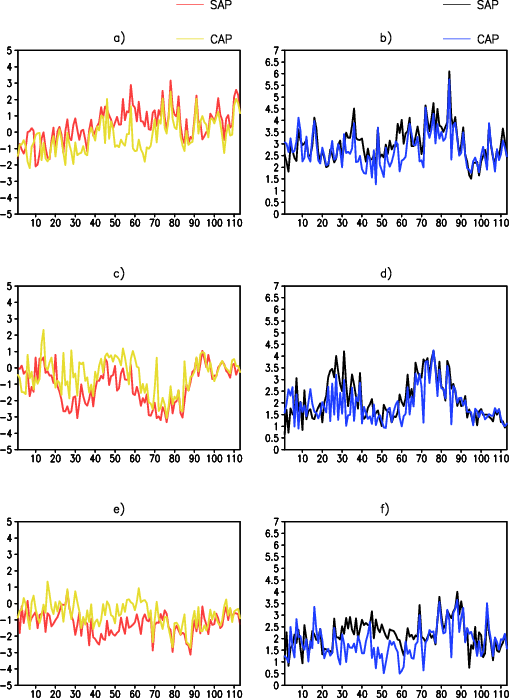
\includegraphics[height=15cm]{./figs/vies_eqm-temp.png}
\caption{Idem Figura 2.3, para a Temperatura do Ar [ºC].}
\label{fig44}
\end{figure}

\begin{figure}[!hbp]
\centering
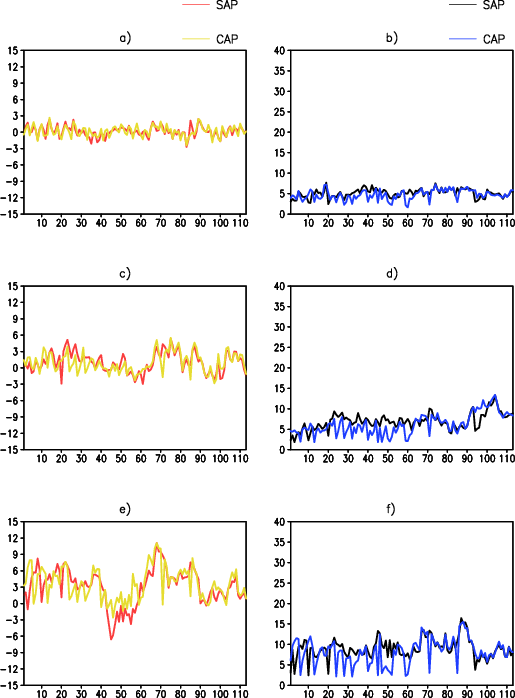
\includegraphics[height=15cm]{./figs/vies_eqm-uvel.png}
\caption{Idem Figura 2.3, para o Vento Zonal [ms-1].}
\label{fig45}
\end{figure}

\begin{figure}[!hbp]
\centering
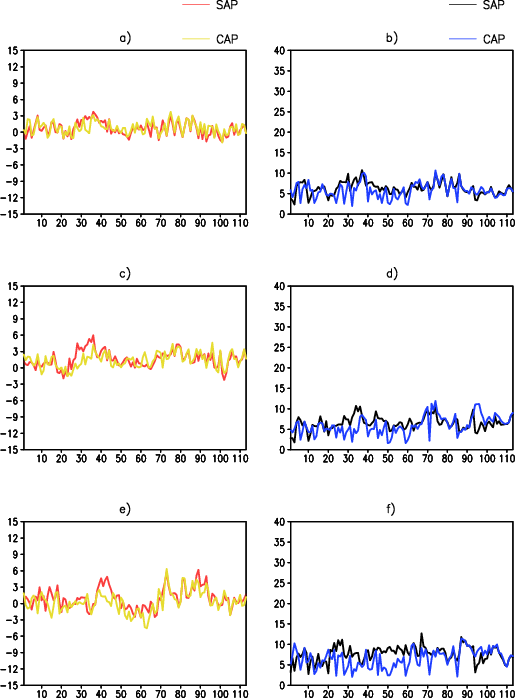
\includegraphics[height=15cm]{./figs/vies_eqm-vvel.png}
\caption{Idem Figura 2.3, para Vento Meridional [ms-1].}
\label{fig46}
\end{figure}

\begin{figure}[!hbp]
\centering
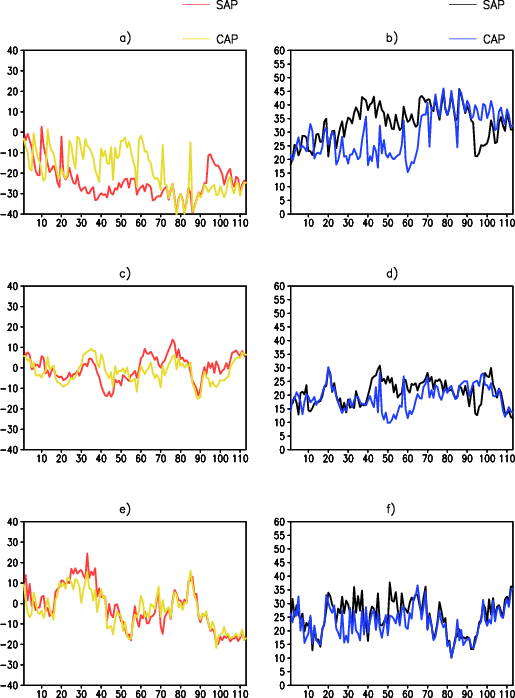
\includegraphics[height=15cm]{./figs/vies_eqm-umrl.png}
\caption{Idem Figura 2.3, para a Umidade Relativa [\%].}
\label{fig47}
\end{figure}

\begin{figure}[!hbp]
\centering
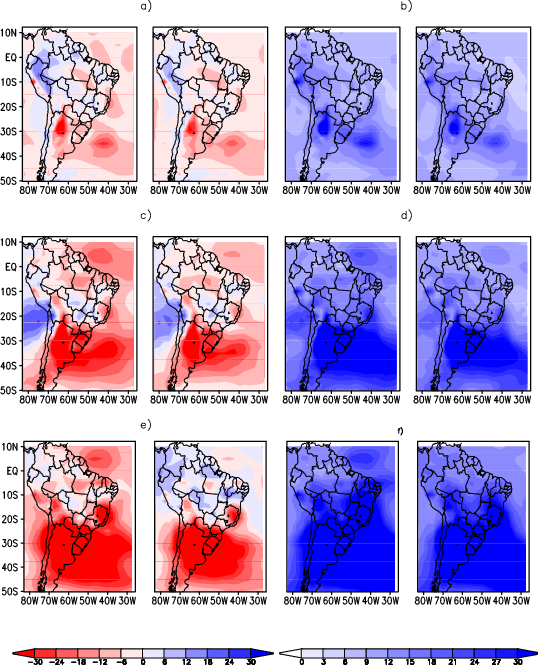
\includegraphics[height=15cm]{./figs/campo_vies_eqm-zgeo.png}
\caption{Viés e EQM espacial da Altura Geopotencial [mgp] para os níveis de a,b) 850 hPa; c,d) 500 hPa e e,f) 250 hPa. As colunas 1 e 3 representam o Viés e o EQM para o experimento SAP, respectivamente. As colunas 2 e 4, representam o Viés e o EQM para o experimento CAP, respectivamente.}
\label{fig48}
\end{figure}

\begin{figure}[!hbp]
\centering
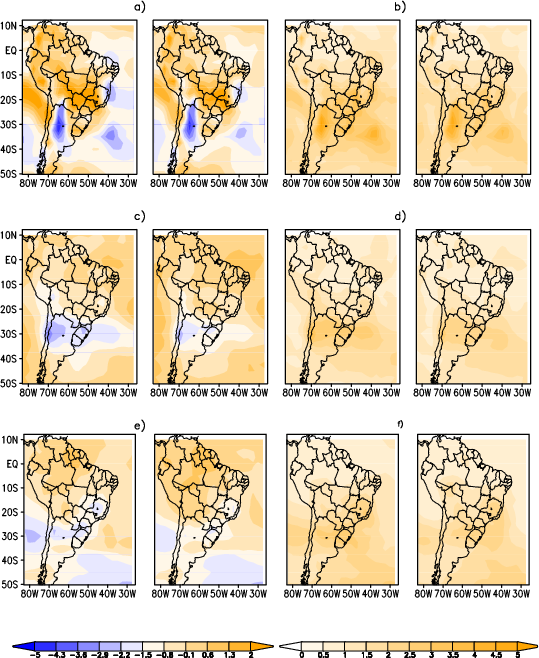
\includegraphics[height=15cm]{./figs/campo_vies_eqm-temp.png}
\caption{Idem Figura 2.8, para a Temperatura Absoluta [ºC].}
\label{fig49}
\end{figure}

\begin{figure}[!hbp]
\centering
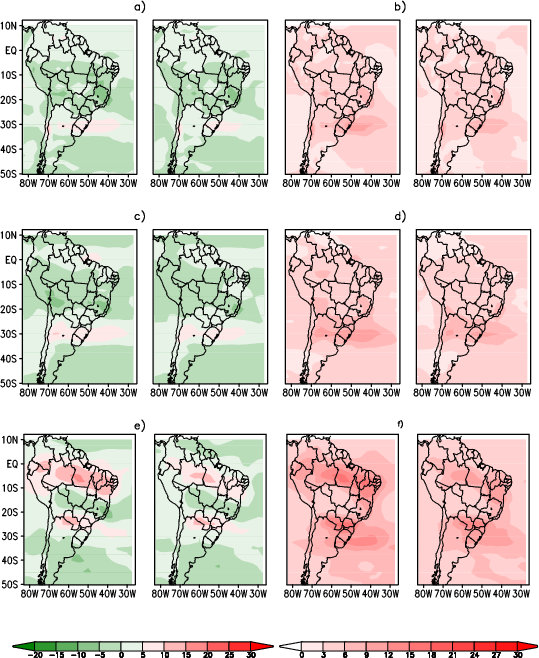
\includegraphics[height=15cm]{./figs/campo_vies_eqm-uvel.png}
\caption{Idem Figura 2.8, para o Vento Zonal [ms-1].}
\label{fig50}
\end{figure}

\begin{figure}[!hbp]
\centering
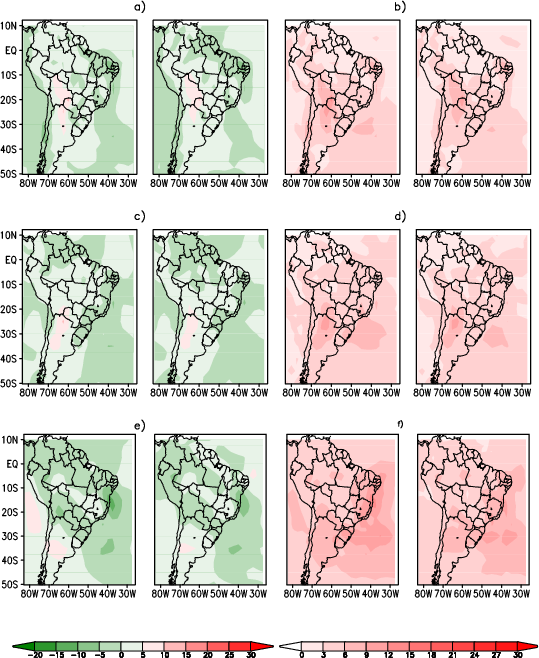
\includegraphics[height=15cm]{./figs/campo_vies_eqm-vvel.png}
\caption{Idem Figura 2.8, para o Vento Meridional [ms-1].}
\label{fig51}
\end{figure}

\begin{figure}[!hbp]
\centering
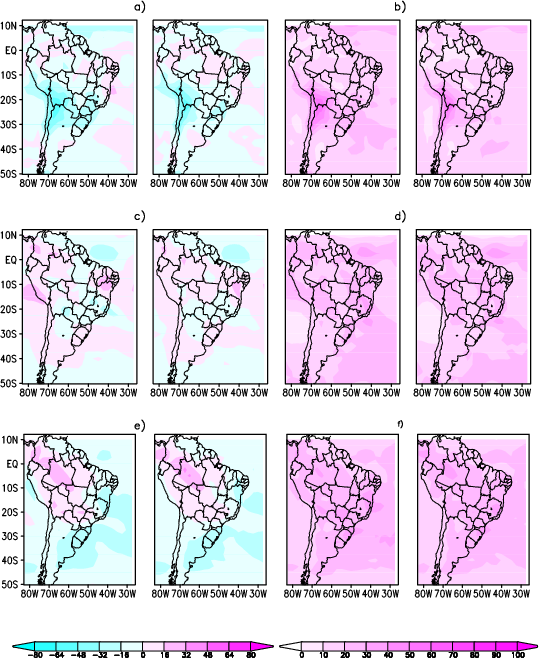
\includegraphics[height=15cm]{./figs/campo_vies_eqm-umrl.png}
\caption{Idem Figura 2.8, para a Umidade Relativa [\%].}
\label{fig52}
\end{figure}

Em relação à temperatura e umidade do solo, a versão do modelo Eta utilizada nos experimentos desta dissertação utiliza o modelo de superfície NOAH para o cálculo destas variáveis. Neste caso as condições iniciais de temperatura e umidade do solo são provenientes do modelo Global do CPTEC T231L42 e são atualizadas a cada dia pelo modelo NOAH. A Figura 3.2 mostra a série temporal da umidade do solo durante o período de integração (de 02 a 30 de Janeiro) do modelo Eta bem como os campos médios.

\begin{figure}[!hbp]
\centering
\includegraphics[height=15cm]{./figs/serie_umidade_solo-ANL.png}
\caption{a) e b) Série temporal da umidade do solo para a área de estudo (BP) e América do Sul (AS), respectivamente. c) e d) Campos médios da umidade do solo para os experimentos SAP e CAP, respectivamente. Linhas vermelha e preta representam o experimento SAP. Linhas amarela e azul, representam o experimento CAP. As unidades estão em kg/s-1.}
\label{fig53}
\end{figure}

Nesta figura são mostradas as séries temporais da umidade do solo (entre 0 e 10 cm - primeira camada) (a) para os experimentos SAP e CAP, tanto para o domínio de integração do modelo (AS) quanto para a região de estudo (BP). Comparando-se os experimentos SAP e CAP, nota-se que o experimento CAP apresenta valores de umidade mais elevados do que o experimento SAP. Numericamente, a maior diferença entre as séries temporais é de ~0,08 kg/m-2.

Em relação à temperatura do solo (Figura 3.4), também observou-se que o experimento CAP apresentou valores diferentes em relação ao experimento SAP. Em média, estes valores não diferem muito (imagens “c” e “d” da Figura 3.4), sendo que menores valores podem ser encontrados na série do experimento CAP (linhas amarela e azul das imagens “a” e “b”), tanto para a área de estudo (BP) quanto para o domínio de integração (AS).

\begin{figure}[!hbp]
\centering
\includegraphics[height=15cm]{./figs/serie_temperatura_solo-ANL.png}
\caption{Idem Figura 3.3, para a Temperatura do Solo. As unidades estão em ºC.}
\label{fig54}
\end{figure}

\subsubsection{Avaliação do Skill do modelo Eta para as previsões de 6 a 24 horas}

Na figura 4.1.1 apresenta-se o Viés, EQM e CA da altura geopotencial para os horários das 00Z (coluna da esquerda) e 12Z (coluna da direita) para as previsões de 0 a 24 horas, no nível de 850 hPa. No geral nota-se que o experimento CAP apresenta resultados um pouco melhores no horário das 00Z durante 0 e 12 horas de previsão (figuras da coluna da esquerda) do que no horário das 12Z. No entanto, às 12Z (figuras da coluna direita) nota-se que entre 12 e 18 horas de previsão o experimento CAP apresenta resultados um pouco melhores. Isso pode ser devido ao fato de que às 12Z a quantidade de observações sinótica é um pouco mais abundante do que às 00Z. Além disso, este resultado indica que o modelo se ajustou aos dados de precipitação assimilados, se comparado com o viés presente em 6 horas de previsão e em comparação com o experimento de controle SAP, que neste mesmo horário apresenta viés quase igual a zero. Em relação ao desempenho, embora os valores de CA se apresentem aquém em relação ao que se conhece do modelo operacional Eta do CPTEC – mas considerando-se a metodologia apresentada, nota-se que o desempenho do experimento CAP, na média, foi melhor no horário das 12Z do que às 00Z. Novamente, isto pode ser devido ao fato de haver uma maior abundância de dados sinóticos assimilados na análise das 12Z, o que levou o modelo a se ajustar mais rapidamente aos dados de precipitação assimilados pelo EtaWS.

\begin{figure}[!hbp]
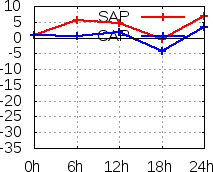
\includegraphics[height=5.5cm]{./figs/VIES850zgeo0Z.png}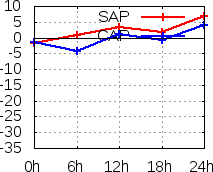
\includegraphics[height=5.5cm]{./figs/VIES850zgeo12Z.png}
\includegraphics[height=5.5cm]{./figs/EQMzgeo0Z.png}\includegraphics[height=5.5cm]{./figs/EQMzgeo12Z.png}
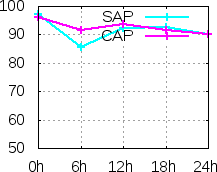
\includegraphics[height=5.5cm]{./figs/CA850zgeo0Z.png}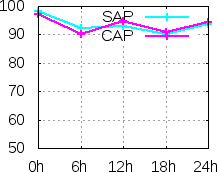
\includegraphics[height=5.5cm]{./figs/CA850zgeo12Z.png}
\caption{Viés, EQM e CA para a variável altura geopotencial em 850 hPa. A coluna da esquerda mostra os valores das medidas para o horário das 00Z. A coluna da esquerda mostra os valores das medidas para o horário das 12Z.}
\label{fig09}
\end{figure}

A próxima figura (\autoref{fig10}) mostra os valores dos índices estatísticos para a altura geopotencial no nível de 500 hPa.

\begin{figure}[!hbp]
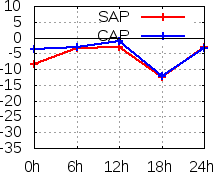
\includegraphics[height=5.5cm]{./figs/VIES500zgeo0Z.png}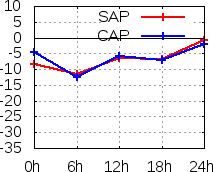
\includegraphics[height=5.5cm]{./figs/VIES500zgeo12Z.png}
\includegraphics[height=5.5cm]{./figs/EQMzgeo0Z.png}\includegraphics[height=5.5cm]{./figs/EQMzgeo0Z.png}
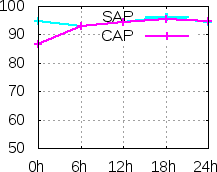
\includegraphics[height=5.5cm]{./figs/CA500zgeo0Z.png}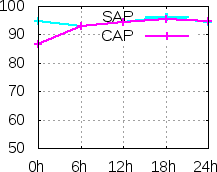
\includegraphics[height=5.5cm]{./figs/CA500zgeo0Z.png}
\caption{Viés, EQM e CA para a variável altura geopotencial em 500 hPa. A coluna da esquerda mostra os valores das medidas para o horário das 00Z. A coluna da esquerda mostra os valores das medidas para o horário das 12Z.}
\label{fig10}
\end{figure}

Analisando-se o a altura geopotencial no nível de 500 hPa, observa-se que os valores de viés para ambos os experimentos tendem a ser negativos durante todo o período de previsão (de 0 a 24 horas). Isto significa os experimentos SAP e CAP subestimaram o valor do geopotencial em níveis médios fazendo com que os valores do EQM aumentassem de 10 mgp para valores entre 20 e 30 mgp. Observa-se um distanciamento sensível dos valores apresentados pelos experi-mentos em relação à Reanálise em 18 horas de previsão, no horário das 00Z. Este diferença é refletida nos valores do EQM, mas não afeta o desempenho geral do experimento CAP que, durante as 24 horas de previsão, apresentou pequena diferença em relação ao experimento de controle SAP. No horário das 12Z, o experimento CAP mostra-se melhor durante as 24 horas de previsão. Aparentemente, a quantidade de dados sinóticos assimilados, influencia a composição do campo de geopotencial pelo modelo, sendo (a priori) um indicativo da necessidade de mais dados de observação para a melhoria da condição inicial do modelo. Tanto em 850 hPa (\autoref{fig09}) quanto em 500 hPa (\autoref{fig10}), para o horário das 12Z, nota-se uma convergência dos valores de CA em 12 horas de previsão, o que pode ser atribuído a uma falha no campo de pre-cipitação associado (um dado faltante no horário da previsão).

Em todos os dois experimentos analisados (SAP e CAP), utilizou-se como condição inicial a análise do NCEP. Posteriormente, após o primeiro ciclo de previsões, o próprio sistema EtaWS+RPSAS gerou a análise utilizada nos ciclos subsequentes. Na avaliação destes resultados utiliza-se também um produto puramente de modelagem que é a Reanálise. Comparar dados de previsão, que embora sejam corrigidos por observações sinóticas, mas que tendem a se distanciar da verdade com o passar do tempo, pode ser tendencioso no sentido de se onerar a quali-dade das previsões dos experimentos e dar mais peso à modelagem. Isso pode acontecer porque a Reanálise se utiliza de dados modelados para reproduzir o estado passado da atmosfera, quase que de forma inversa ao que é feito com a previsão de tempo, onde se utiliza dados ob-servados para se representar o estado presente ou futuro da atmosfera. Com isso, o produto que se obtém da Reanálise possui uma qualidade muito grande porque nela está contida a maior quantidade possível de dados observados que, em comparação à realidade dos experimentos, pode não ser verdade.

A seguir (\autoref{fig11}) são apresentados os resultados do Viés, do EQM e da CA para a temperatura do ar.

\begin{figure}[!hbp]
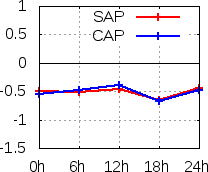
\includegraphics[height=5.5cm]{./figs/VIES850temp0Z.png}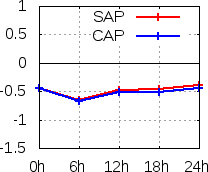
\includegraphics[height=5.5cm]{./figs/VIES850temp12Z.png}
\includegraphics[height=5.5cm]{./figs/EQMtemp0Z.png}\includegraphics[height=5.5cm]{./figs/EQMtemp12Z.png}
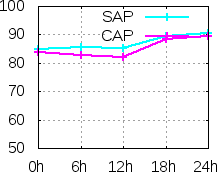
\includegraphics[height=5.5cm]{./figs/CA850temp0Z.png}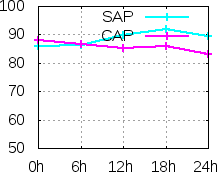
\includegraphics[height=5.5cm]{./figs/CA850temp12Z.png}
\caption{Viés, EQM e CA para a variável temperatura do ar em 850 hPa. A coluna da esquerda mostra os valores das medidas para o horário das 00Z. A coluna da esquerda mostra os valores das medidas para o horário das 12Z.}
\label{fig11}
\end{figure}

A avaliação dos índices estatísticos considerados para a variável temperatura em 850 hPa, su-gere que, no geral, o experimento CAP tende a subestimar mais os valores de temperatura ao longo de 24 horas de previsão, tanto às 00Z quanto às 12Z do que o experimento SAP. Este resultado se reflete diretamente nos valores do EQM, principalmente durante as 12 primeiras horas de previsão. Este resultado pode ser associado ao fato de que há menos observações de temperatura no horário das 00Z do que no horário das 12Z. Outro fator que pode ser associado a este resultado é a dependência de que a precipitação tem dos processos de escala de subgrade, seja na liberação de calor latente ou na modulação do perfil vertical de umidade, o qual a tempe-ratura está associada.

A assimilação de precipitação pelo modelo EtaWS é um processo de inicialização física, onde as variáveis prognósticas do modelo são inicializadas de acordo com as alterações nos perfis verticais de calor e umidade. Estes perfis são alterados quando se compara a precipitação produzida pelo modelo em relação à precipitação observada (conforme explicado no \autoref{assimprec} na \autoref{tab02}). A temperatura é uma das variáveis que são diretamente influenciadas pelas alterações nos perfis de calor e umidade, devido à sua condição de referência no esquema de convecção. 

A CA da temperatura para o horário das 00Z é menor para o experimento CAP nas 12 primeiras horas de previsão e tendem a ser maior nas últimas 12 horas, em comparação ao experimento SAP. No horário das 12Z observa-se o contrário, sendo o experimento CAP melhor do que o experimento SAP nas 12 primeiras horas de previsão.

As \autoref{fig12} e \autoref{fig13}, mostram os valores dos índices de Viés e EQM para a temperatura do ar nos níveis de 500 e 250 hPa. Em médios e altos níveis, observa-se que o viés da temperatura tende a apresentar um comportamento semelhante ao apresentado em baixos níveis, reforçando a idéia de que a temperatura é sensível às alteração de calor e umidade. No entanto, enquanto que em médios níveis, no horário das 12Z o EQM da temperatura tende a ser pequeno, em altos níveis este erro é muito grande e chega a ser uma ordem de grandeza maior. Em geral, observa-se que o experimento CAP subestima menos os valores de temperatura do que o experimento SAP. A CA da temperatura para esses níveis foi omitida por não apresentar resultados relevantes.
     
\begin{figure}[!hbp]
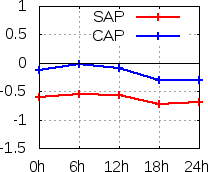
\includegraphics[height=5.5cm]{./figs/VIES500temp0Z.png}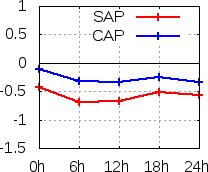
\includegraphics[height=5.5cm]{./figs/VIES500temp12Z.png}
\includegraphics[height=5.5cm]{./figs/EQMtemp0Z.png}\includegraphics[height=5.5cm]{./figs/EQMtemp12Z.png}
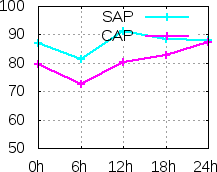
\includegraphics[height=5.5cm]{./figs/CA500temp0Z.png}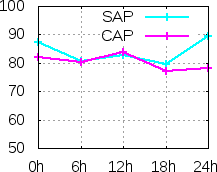
\includegraphics[height=5.5cm]{./figs/CA500temp12Z.png}
\caption{Viés, EQM e CA para a variável temperatura do ar em 500 hPa. A coluna da esquerda mostra os valores das medidas para o horário das 00Z. A coluna da esquerda mostra os valores das medidas para o horário das 12Z.}
\label{fig12}
\end{figure}

\begin{figure}[!hbp]
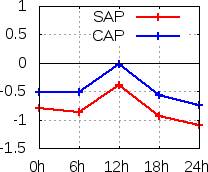
\includegraphics[height=5.5cm]{./figs/VIES250temp0Z.png}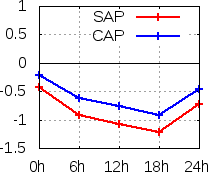
\includegraphics[height=5.5cm]{./figs/VIES250temp12Z.png}
\includegraphics[height=5.5cm]{./figs/EQMtemp0Z.png}\includegraphics[height=5.5cm]{./figs/EQMtemp12Z.png}
\includegraphics[height=5.5cm]{./figs/CA250temp0Z.png}\includegraphics[height=5.5cm]{./figs/CA250temp12Z.png}
\caption{Viés, EQM e CA para a variável temperatura do ar em 250 hPa. A coluna da esquerda mostra os valores das medidas para o horário das 00Z. A coluna da esquerda mostra os valores das medidas para o horário das 12Z.}
\label{fig13}
\end{figure}